\documentclass[fontsize=28pt,a4paper]{scrartcl}

\usepackage[margin=0.75in,includefoot,bottom=0.3in,footskip=2em]{geometry}

\usepackage{fontspec}
\setmainfont{EBGaramond}
[
  Extension      = .otf ,
  UprightFont    = *-Regular,
  ItalicFont     = *-Italic,
  BoldFont       = *-Bold,
  BoldItalicFont = *-BoldItalic,
  Numbers        = Lowercase,
  Ligatures      = Discretionary,
  Style          = Swash
]
% https://texnique.fr/osqa/questions/8423/lualatex-et-ligatures

\usepackage[french]{babel}

% https://tex.stackexchange.com/a/123669/295527
%\renewcommand*{\FrenchLabelItem}{$\bullet$}
%\frenchsetup{StandardItemLabels=true}
\frenchsetup{StandardLayout=true}

\usepackage{microtype}

\usepackage{xcolor}
\usepackage{tikz}
\usetikzlibrary{intersections,calc}
\usepackage{caption}

\usepackage[showmarks]{pocketmod}% https://github.com/liantze/pocketmod.sty

% https://fr.overleaf.com/latex/examples/mini-livre-trigonometrie/ntgbdvthxhnb
% https://fr.overleaf.com/latex/examples/mini-livre-exercices-de-rentree-en-seconde/gncxgskzswtc
% https://forge.apps.education.fr/duplessyerwan/site-mini-math-livre

\usepackage{graphicx}
\usepackage{enumitem}
\setlist{leftmargin=\parindent,labelindent=*}
\usepackage{hyperref}
\usepackage[hyphenbreaks]{breakurl}

%\title{Creating PocketMods with \LaTeX}
\title{Socrate et la justice}

%\author{LianTze Lim}
%\author{\small Vincent Pantaloni}
\author{\small R. Chastain}
\date{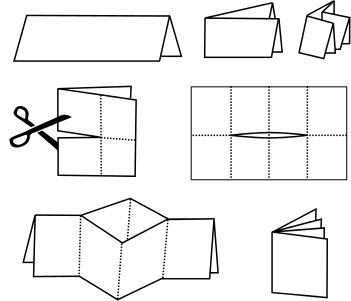
\includegraphics[width=.75\textwidth]{folding-minibook}}

\begin{document}

\maketitle
\thispagestyle{empty}
\clearpage

\section{Le procès}

En 399 av. J.-C., Socrate comparaît devant un tribunal d'Athènes. On l'accuse de corrompre la jeunesse et de professer l'athéisme. On dit de lui, d'après une comédie du poète Aristophane, qu'il possède l'art de donner au mensonge les couleurs de la vérité.

On lui reproche encore que son ancien disciple Critias soit devenu l'un des Trente Tyrans. Pourtant, sous l'oligarchie sanglante des Trente, Socrate a montré une liberté dans ses discours. Il a refusé d'arrêter Léon de Salamine, désobéissant au risque de sa vie à un ordre qu'il estimait illégal.

% Quand vint l’oligarchie, les Trente me donnèrent l’ordre d’amener de Salamine Léon le Salaminien, afin qu’on le fît mourir ; car ils donnaient de pareils ordres à beaucoup de personnes, pour compromettre le plus de monde qu’ils pourraient ; et alors je prouvais, non pas en paroles, mais par des effets, que je me souciais de la mort comme de rien, si vous me passez cette expression triviale, et que mon unique soin était de ne rien faire d’impie et d’injuste. Toute la puissance des Trente, si terrible alors, n’obtint rien de moi contre la justice.
% ... les quatre autres s’en allèrent à Salamine, et amenèrent Léon, et moi je me retirais dans ma maison ; et il ne faut pas douter que ma mort n’eût suivi ma désobéissance, si ce gouvernement n’eût été aboli bientôt après. C’est ce que peuvent attester un grand nombre de témoins.
% ... ne cédant jamais rien à qui que ce soit contre la justice, non pas même à aucun de ces tyrans, que mes calomniateurs veulent faire passer pour mes disciples.

Socrate estime mériter d'être nourri au prytanée. La plupart des juges se tiennent si offensés de la franchise \& de la noble hardiesse avec laquelle il leur a parlé, qu'ils le condamnent à mort.

% d'avoir toute l'attention possible à ceci, c'est-à-savoir si je vous dis des choses justes, car c'est en cela que consiste la vertu du Juge, comme celle de l'Orateur consiste à ne dire que la vérité.

% pour ne pas demeurer court, ils ont recours à ces reproches triviaux qu'on fait ordinairement aux Philosophes, qu'ils recherchent ce qui se passe dans les cieux et dans le sein de la terre ; qu'ils ne croient point de Dieux, et qu'ils rendent bonnes les plus méchantes causes

%\frquote{Mais il est temps que nous nous quittions, moi pour mourir, et vous pour vivre. Qui de nous a le meilleur partage ? Personne ne le sait, excepté Dieu.}
% https://remacle.org/bloodwolf/philosophes/platon/cousin/apologie.htm

\clearpage

\section{L'oracle de Delphes}

À en croire Socrate, il n'y a pas un mot de vrai dans ces accusations. La vraie raison qui anime contre Socrate ses calomniateurs, c'est qu'il a dévoilé leur ignorance. C'est pour cela qu'on en veut à Socrate. Il y a une infinité de gens qui croient savoir quelque chose, et qui ne savent rien. Ceux que Socrate a confondus s'en prennent à lui, et disent qu'il corrompt la jeunesse.

Ce qui a conduit Socrate dans cette voie périlleuse, c'est le désir de comprendre l'oracle : l'oracle qui, à l'audacieuse question de Chéréphon, a répondu, par la bouche de la Pythie, que Socrate était le plus sage des hommes.

Quand Socrate apprend ce que l'oracle a dit à son sujet, il est étonné, parce qu'il ne croit pas savoir plus de choses que les autres. Il ne croit pas non plus que la Divinité puisse mentir. Il se demande simplement quel est le sens de l'oracle.

%\frquote{Quand je sus la réponse de l'oracle, je pensai en moi, que veut donc
%dire le Dieu ? Quel sens caché y a-t-il sous ces paroles ? Car je sais
%bien qu'il n'y a en moi aucune sagesse, ni petite, ni grande ; que
%veut-il donc dire en me déclarant le plus sage des hommes ? Car il ne ment point, la Divinité ne saurait mentir.}

\clearpage

\section{La sagesse humaine}

\frquote{Or il me semble, Athéniens, qu'il n'y a que Dieu seul qui soit véritablement
sage, et que c'est aussi ce qu'il a voulu dire par son oracle, en
faisant entendre que toute la sagesse humaine n'est pas grand'chose, ou
pour mieux dire qu'elle n'est rien. Il s'est sans doute servi de mon nom pour me proposer en
exemple, comme disant à tous les hommes, \textit{le plus sage d'entre vous,
c'est celui qui reconnaît comme Socrate, qu'il n'y a véritablement
aucune sagesse en lui.}}

\frquote{Pour moi je suis en cela bien différent de tous les autres hommes. Et si
je parais plus sage qu'eux en quelque chose, c'est en ce que ne sachant
pas bien ce qui se passe dans les enfers, je ne crois pas non plus le
savoir. La seule chose que je sais, c'est que commettre des injustices
et de désobéir à ce qui est meilleur que nous et au dessus de nous, soit
Dieu, soit homme, il n'y a rien de plus criminel ni de plus honteux.}

%{\centering
%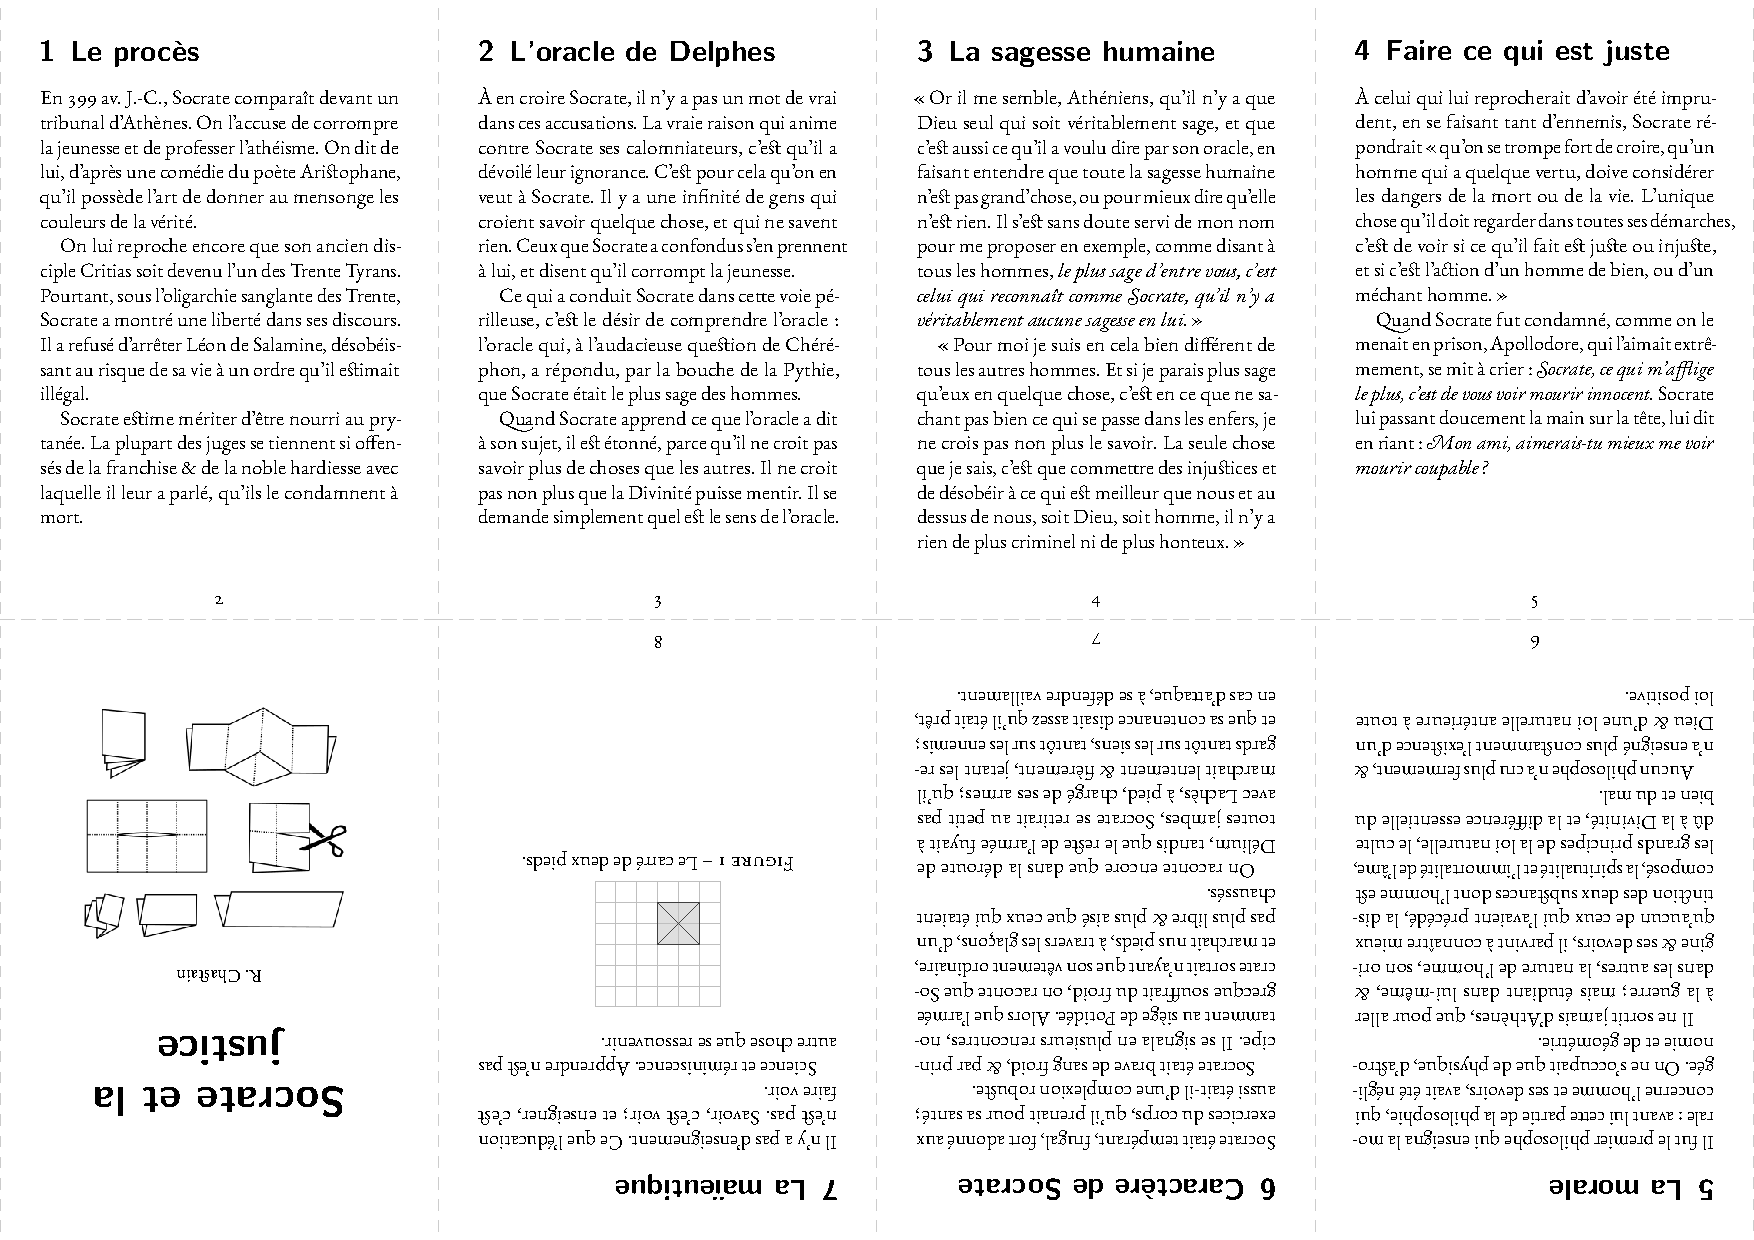
\includegraphics[width=\textwidth]{socrate}
%\par
%}

\clearpage

\section{Faire ce qui est juste}

À celui qui lui reprocherait d'avoir été imprudent, en se faisant tant d'ennemis, Socrate répondrait \frquote{qu'on se trompe fort de croire, qu'un
homme qui a quelque vertu, doive considérer les dangers de la mort ou de
la vie. L'unique chose qu'il doit regarder dans toutes ses démarches,
c'est de voir si ce qu'il fait est juste ou injuste, et si c'est
l'action d'un homme de bien, ou d'un méchant homme.}

Quand Socrate fut condamné, comme on le menait en prison, Apollodore, qui l'aimait extrêmement, se mit à crier : \textit{Socrate, ce qui m'afflige le plus, c'est de vous voir mourir innocent.} Socrate lui passant doucement la main sur la tête, lui dit en riant : \textit{Mon ami, aimerais-tu mieux me voir mourir coupable ?}

\clearpage

\section{La morale}

Il fut le premier philosophe qui enseigna la morale : avant lui cette partie de la philosophie, qui concerne l'homme et ses devoirs, avait été négligée. On ne s'occupait que de physique, d'astronomie et de géométrie.

Il ne sortit jamais d'Athènes, que pour aller à la guerre ; mais étudiant dans lui-même, \& dans les autres, la nature de l'homme, son origine \& ses devoirs, il parvint à connaître mieux qu'aucun de ceux qui l'avaient précédé, la distinction des deux substances dont l'homme est composé, la spiritualité et l'immortalité de l'âme, les grands principes de la loi naturelle, le culte dû à la Divinité, et la différence essentielle du bien et du mal.

Aucun philosophe n'a cru plus fermement, \& n'a enseigné plus constamment l'existence d'un Dieu \& d'une loi naturelle antérieure à toute loi positive.

%{\centering
%\includegraphics[width=.5\textwidth]{IMG_2822}%
%\par
%}

\clearpage

\section{Caractère de Socrate}

Socrate était tempérant, frugal, fort adonné aux exercices du corps, qu'il prenait pour sa santé ; aussi était-il d'une complexion robuste.

Socrate était brave de sang froid, \& par principe. Il se signala en plusieurs rencontres, notamment au siège de Potidée. Alors que l'armée grecque souffrait du froid, on raconte que Socrate sortait n'ayant que son vêtement ordinaire, et marchait nus pieds, à travers les glaçons, d'un pas plus libre \& plus aisé que ceux qui étaient chaussés.

On raconte encore que dans la déroute de Délium, tandis que le reste de l'armée fuyait à toutes jambes, Socrate se retirait au petit pas avec Lachès, à pied, chargé de ses armes ; qu'il marchait lentement \& fièrement, jetant les regards tantôt sur les siens, tantôt sur les ennemis ; et que sa contenance disait assez qu'il était prêt, en cas d'attaque, à se défendre vaillament.

\clearpage

\section{La maïeutique}

Il n'y a pas d'enseignement. Ce que l'éducation n'est pas. Savoir, c'est voir ; et enseigner, c'est faire voir.

Science et réminiscence. Apprendre n'est pas autre chose que se ressouvenir.

\begin{figure}[h]
  \centering
  \begin{tikzpicture}%[scale=0.5]
    \draw[step=1cm,lightgray,very thin] (0,0) grid (6,6);
    \fill[lightgray,opacity=0.5] (1,1) rectangle (3,3);
    \draw[darkgray,thick] (1,1) -- (1,3) -- (3,3) -- (3,1) -- cycle;
    \draw[darkgray,thick] (1,1) -- (3,3);
    \draw[darkgray,thick] (1,3) -- (3,1);
  \end{tikzpicture}
  \caption{Le carré de deux pieds.}
\end{figure}

\end{document}
